\part{Cross correlation of exoplanet spectra from high contrast imaging data for simulataneous detection and characterization}
%\vfill
\startcontents[chapters]
\printmyminitoc{}
\chapter{Cross correlation for processing exoplanet spectra}
\label{chap:II.1}
\section{Introduction to cross correlation of spectra}
\section{Adapting the cross correlation function to detecting exoplanets}
\section{Interpretation of cross correlation values}

\chapter{Spectral data generation to test the effectiveness of cross correlation based detection and characterization}
\label{chap:II.2}
Spectra have a wide range of properties, such as $\rm{SNR}$, line width etc. and we need to choose properties that are in line with science goals of detection and characterization.
The goal of this chapter is to define,
\begin{itemize}
    \item the scientific objective of using HCI spectra,
    \item the data that we will use to achieve these objectives and
    \item the metric that will be used to state whether this chosen objective was met or not.
\end{itemize}
In that quest we structure this chapter to start with introducing a science goal by defining the detection and characterization hypothesis.
This will then be followed by describing the parameters chosen for data generation followed by a description of the data generation itself.
This will be followed by describing the benchmark metric formulation.
This chapter aims to set up the basic framework that will be used in the two methods chapters in this part.

\section{Scientific goals of using spectral data to detect and characterize exoplanets}
%Using spectra directly with ML algorithms has not been particularly successful for a specific set of characterization problems \citep[e.g,][]{2020Fisher}.
%In order to not repeat previous studies and to redefine the goals of spectral data processing with ML algorithms we separate our goals as detection and characterization goals.
As stated in the introduction to this part, the goal of this part is to explore the use of cross correlation to detect and characterize exoplanets using their spectra alone.
While detection and characterization are performed with the same spectra their goals can be quite different, thus in this chapter we define them explicitly.
Detection goals pertain to identifying that a spectrum indeed contains spectral features that pertain to an exoplanet.
The characterization goals pertain to using the spectral absorption features to derive constraints on the $\rm{T_{eff}}$ and $\log(\rm{g})$ of the exoplanet in the spectrum.
\subsection{Detection hypothesis}
The detection hypothesis is expressed as the ability to identify an exoplanet spectrum when it is extracted from a pixel of a high contrast image based on the features of the extracted spectrum alone.
In the context of high contrast imaging this means that no matter, the contrast of the exoplanet or the resolution of the spectrograph it is possible to make this fundamental distinction based on the spectral absorption features in the spectrum.

This would prove particularly useful when trying to discriminate between speckles and exoplanets in an residual cube.
A well designed algorithm should be able to test and validate this hypothesis.
%In this part we will develop a ML and a non-ML based algorithm to test this hypothesis.
%We will use the non-ML algorithm to develop the benchmark values that the ML algorithms need to achieve to validate the detection hypothesis.

\subsection{Characterization hypothesis}
The characterization hypothesis is expressed as the ability to constrain physical exoplanetary parameters with a well defined and repeatable error bar when exoplanet spectral features are present in the spectrum.
The exoplanetary parameters that we will consider in my thesis are the $\rm{T_{eff}}$ and $\log(g)$.
In the context of direct imaging data it means that no matter the spectral resolution of the instrument, if exoplanetary spectral features are present in the spectrum then the hypothesis states that we are able to constrain the $\rm{T_{eff}}$ and $\log(\rm{g})$ within the stated error bars. 

This hypothesis is motivated by the idea that it is possible that detection algorithms produce false positives due to their systematic biases. 
However, characterization constraints could allow to rule out such false positives when the detection is marginal.

These two hypotheses form the basis of our data generation, algorithm development and interpretation of those results. 
The detection hypothesis is disproven if we are not able to find the point at which we are not able to make perfect detections no matter the resolution and contrast of the exoplanet present in the spectrum.
The characterization hypothesis is also disproven if we are not able to define the minimum error-bar with which we constrain the $\rm{T_{eff}}$ and $\rm{\log(g)}$.

\section{Data generation to test our hypotheses}
%Testing our detection and characterization hypotheses requires us to have data with sufficient variance in data parameters and with sufficient astrophysical variance.
We have to test both our hypotheses on the same data that has sufficient variance in fundamental parameters, in this section we will define those paramters and the consequent data generation framework.
\subsection{ Choice of parameters for data generation}
We confine ourselves to a smaller set of parameters to study.
We choose three parameters, one of which is entirely intrinsic to the exoplanet we are studying and two of them are intrinsic to the the imaging strategy and the choice of spectrograph.
The parameters we use in this part of the thesis to test our hypotheses are,
 \begin{enumerate}
     \item \textbf{Contrast $~(\mathbf{C})~$:}
     The contrast of an exoplanet is defined as the flux ratio of the mean flux emitted by the exoplanet to mean stellar flux. 
     In principle, the brightness of the exoplanet is a free parameter that varies based on the temperature, composition, atmosphere physics (such as presence of clouds) and environment of the exoplanet. 
     The brightness of the star is mostly driven by its spectral type and surface gravity.
     Therefore, when the brightness of the star is fixed (by knowing accurately its spectral type and surface gravity), the contrast is only influenced by the brightness of the exoplanet in question.
     \item \textbf{Signal to noise ratio of measured spectrum $~(\rm{\mathbf{SNR}})~$:}
     The signal part of a spectrum is a measure of the number of photons in the spectrum that are from an observation (i.e from the star and the planet).
     The noise can be measured in several ways, but the most basic noise that is present in an observation is the photon noise.
     In this part of the thesis, we limit our scope to measuring this noise and thus the signal to noise ratio is a ratio of the observed photons and the photon noise.
     %number of photons received from the exoplanet vs the instrinsic random noise that is naturally present in the data due to the act of observing an exoplanet.
     %This noise is also called photon noise and is usually random in nature.
     %This also relates to the quality of the spectrum in that when we have higher number of photons as compared to the number of intrinsic observational noise present in the data.
     The $\rm{SNR}$ is typically a function of integration time of the observations, such that longer observing times lead to higher $\rm{SNR}$.
     \item \textbf{Resolution of the spectrograph $~(\mathbf{R})~$:}
     The spectral resolution is the ratio of a fixed wavelength to the difference between wavelengths of two consequent wavelength bins.
     $R$ is typically dependent on the instrument and changes with the wavelength in consideration and is typically higher for higher wavelengths.
     To keep the interpretation simple we consider a fixed $R$ as computed for the smallest wavelength in our data.
 \end{enumerate}
%In literature, the $C$ for instance is the single parameter that defines the sensitivity in the data when computing contrast curves,
%the $\rm{SNR}$ is the parameter that is expected to be the limiting factor when developing a new instrument,
%and the $R$ has long been considered the key factor in using spectra in direct exoplanet detection and \citep[e.g KPIC, ][]{2016Mawet} has prided itself on provide high $\rm{SNR}$ and high $R$ spectra.
\subsection{Synthetic spectra library}
To test our hypotheses, these parameters have to be sampled over a large sample space to ensure that we are able to rigorously test our hypotheses.
Additionally, instrument parameters will require us to have access to instruments with different resolutions but we will need to the exoplanets imaged with these instruments at different $\rm{SNR}$ and $C$.
This also implies that we cannot control the types of noise that are present in instruments and we cannot limit our study to just the observation noise.
Using data from different instruments and different observations will also bring into play,
For example, instrument systematics such as the different Strehl ratios produces different amounts of stellar leakages produing variable data.
If we choose just one type of instrument choose to drop $R$ we still risk observation systematics such as different seeing on different nights. 
In addition to other well known effects such as wind halo, these make for a poorly conditioned dataset. 
While in the previous part we sought to verify that our algorithms work with both real and synthetic data, in this part we seek to verify that with working algorithms are our hypotheses valid.

In order to achieve the desired range in the data without taking into account inter-instrument and site variations, we resort to using synthetic data from the well known template library, \citep[\textsc{BT-SETTL},][]{1997Allard,2011Allard}.
\textsc{BT-SETTL} conveniently also presents us with a simulation tool \citep[\textsc{PHOENIX},][]{2011Allard} that allows us generate accurate atmospheric spectra by specifying the exoplanet properties.
These models sample the $\rm{T_{eff}}$ range from $1200$K corresponding to warm Jupiter type of exoplanets to $7000$K corresponding to the B supergiant spectral type.
The wavelength range varies from $0.1$ $\mu$m up to $16$ $\mu$m i.e from the infra red to the near visible spectrum. 
This allows to simulate the stellar spectrum and the exoplanet spectrum from the same library.
Using BT-SETTL, we choose a basic grid of models and we generate synthetic from this grid depending on the requirement.
The grid is defined by the following parameters,
\begin{itemize}
    \item[] $\rm{\mathbf{T_{eff}}}$: The exoplanet atmosphere is chosen to be between $1200\le \rm{T_{eff}}\le 1900$ K with a grid sampled every $100$K. 
    This range corresponds to that of warm Jupiters. 
    These temperatures do not lend to very pronounced $\rm{CO}$ emissions, which are quite prominent at higher temperatures which make those templates somewhat easier to detect for cross correlations. 
    The star is chosen to have a $5000\le \rm{T_{eff}}\le 7000$ K surface temperature, the choice of temperature is not so relevant for this problem because beyon a temperature of $4000$ K all of the molecules are fully ionized and the $\rm{T_{eff}}$ only impacts the continuum. 
    In our processing we remove the continuum and hence it does not play a part in the analysis.
    \item []$\rm{\mathbf{log(g)}}$: We choose values for the exoplanet within the existing BT-SETTL model to provide enough range to make an error bar estimate. 
    We choose $2.5\le \rm{\log(g)} \le 5.5$ for the exoplanet with a grid sampling rate of $0.5$ dex. 
%j    These $\rm{\log(g)}$s are considerably higher than what we would see for a planet of this type.
    The stellar $\rm{\log(g)} = 2.5$ which is the solar $\rm{\log(g)}$.
    \item []\textbf{Wavelength $\rm{\mathbf{\lambda}}$:} We choose wavelength ranges that allow us to probe the full near infra-red region, $1 \mu\rm{m} \le \lambda \le 3 \mu \rm{m}$.
    This also includes the Telluric absorption lines between $1.78$ and $2.1$ $\mu$m.
    The default spectral resolution of the data $R>300,000$ and the linewidth is in $\AA$, this is downsampled to match the data that we will use througout this thesis.
    We resample the $R$ as needed but we broaden the line width to match an instrumental profile so that the absorption line widths are realistic.
    We choose this width to be the same as the SINFONI instrumental line width.
\end{itemize}
For the rest of this thesis, these \textsc{BT-SETTL} parameters remain pretty much unaltered, unless we use it with data that demands a different template set.

 \section{Generating synthetic spectra}
The goal of our tests is to ascertain the constraints on detection and characterization of exoplanets using a cross correlation based algorithm with direct imaging spectra.
Consequently, the goals of generating synthetic spectra are also two fold, 
\begin{enumerate}
    \item to be able to explore a parameter space which is relevant from both the astronomical as well as signal processing point of view.
    This will allow us to the test the hypotheses and to understand the interplay between the parameters.
    This is relevant to the community to understand if, of the three parameters we have chosen, are there any which play an important role in validating these hypotheses.
    %\item To generate a large number of samples that can be used to train, validate and test the machine learning algorithms that are developed to test our hypotheses.
    %In addition to ML algorithms needing a large number of samples to train and generalize well, we also need this parameter space well sampled in order to derive insights into the performance of the ML algorithms on this data.
    %As in the case of a cross correlation based algorithm, the community will benefit if we are able to derive the limits at which these hypotheses were satisfied by ML algorithms.
    \item to be able to test our algorithms to the limit of what they can achieve for each hypothesis from a scientific point of view.
\end{enumerate}
Thus to generate spectra that are astronomically relevant, having realistic observation noise and finally lend to re derivation of the parameters (i.e now they can be viewed as parameters that can be re-estimated by an observer), we generate the same in three steps.
We split the description of this into three subsections, first we create noise-less spectrum from a combination of stellar and exoplanetary spectrum.
We then follow this with explaining the noise injection process and finally we describe the re-derivation of the $\rm{SNR}$ from this noisy spectrum.
\subsection{Creating astronomically accurate synthetic spectra}
The stellar flux (of the spectrum chosen from BT-SETTL) is measured as $F_{\rm{\lambda,star}}$.
For the exoplanetary spectrum, an exoplanetary template spectrum is randomly chosen with a $1200 \le \rm{T_{eff}} \le 1900$ K and  $2.5 \le \rm{\log(g)}\le  5.5$. 
Both spectra are first downsampled to a desired $R$ such that $10^3<R<10^5$.
Downsampling is a two step process,
\begin{enumerate}
    \item a wavelength vector is first generated with the desired wavelength range where we want to test our hypotheses. 
    In this case we choose $1\le \lambda\le 3$ $\mu$m which falls in the far infrared spectrum and importantly covers all of the major carbon absorption lines. 
    The $R$ of this wavelength is set to the value we choose to generate our synthetic spectra.
    \item We then interpolate a new synthetic spectrum for the specified wavelength bins based on the flux present in the template library.
    Note that the maximum resolution cannot exceed the spectral resolution of the \textsc{BT-SETTL} library ($3\times10^{5}$)
\end{enumerate}
We want to now make sure that every bin has exactly the same relative number of photons so that the sum of all the photons in each of the bins is the same for every spectrum.
Once again to achieve this we have a two step proces, the first of which is normalization.
\paragraph{Normalization:}
Normalization of the flux per wavelength bin ($F_\lambda$) is performed so that the average flux in the spectrum is $1$.
\begin{equation}
    F_\lambda = \dfrac{F_\lambda}{\sum\limits_{\lambda} F_{\lambda}}
\end{equation}
Thus, when we do this for the stellar and the exoplanet spectrum we have,
\begin{equation}
     F_{\rm{planet,\lambda,normalized}} =  F_{\rm{star},\lambda,normalized} = 1
\end{equation}
Thus both the star and planet are at the same flux. 
%For ease of notation we drop the word normalized from here on with the understanding that all of the spectrum from this point on is normalized.
%The choice of the number of total photons in the spectrum is related to the flux that we are expected to receive at the telescope when observing the spectra.
%Therefore, we rescale all the spectra to a specific flux level that is proportional to the $\rm{SNR}$ expected to be recovered.
\paragraph{Scaling the spectra:}
We rescale both the $F_{\rm{\lambda,star}}$ and the $F_{\rm{\lambda,planet}}$ with appropriate flux values.
Starting with the star, we scale the stellar flux as
\begin{equation}
    F_{\rm{star,\lambda,new}} = F_{\rm{star,\lambda,normalized}}\times\rm{SNR}^2
    \label{eq:scaling of F}
\end{equation}
The exoplanet usually has a total flux that is proportionally scaled to the stellar flux.
%Note that while the exoplanet has a blackbody temperature, we concern ourselves only with the reflected stellar flux from the exoplanet.
%The absoprtion lines in the exoplanet spectrum are solely due to the presence of specific atmospheric molecules which absorb this reflected light.
The flux from the exoplanet is just a fraction of the stellar flux, expressed usually as a ratio of total planetary flux to the stellar flux known as the contrast $C$.
%This flux ratio of the exoplanet to the star is $C$
Thus exoplanetary flux is expressed as,
\begin{equation}
    F_{\rm{planet},\lambda,new} = C\times F_{\rm{planet},\lambda,normalized}\times \rm{SNR}^2
    \label{eq:exoplanet flux}
\end{equation}
where $C\ll1$.
%Note that when we compute the rescaled new fluxes of the exoplanet to the star we have,
%\begin{equation}
 %   \dfrac{F_{\rm{planet,\lambda,new}}}{F_{\rm{star,\lambda,new}}} = C
  %  \label{eq: defn of contrast}
%\end{equation}
%Thus, the flux of planet to the star defines our contrast as per the definition.
Once the two fluxes have been computed, they have now to be combined and `observed' by a `telescope'.
This act of observation will result in noise, this now the second step to generating synthetic spectra.
\subsection{Noisy spectra generation}
%We now have two spectra that have scaled flux values. 
%We have yet to combine them to form a single spectrum as in an astronomical observation.
In order to simulate an observation where we extract a spectrum from an observed pixel, we combine both the stellar and planetary spectra as,
 \begin{equation}
     F_{\rm{total},\lambda}=(1-C)F_{\rm{star},\lambda,new} + F_{\rm{planet},\lambda,new}
     \label{eq:insertion}
 \end{equation}
Thus, $F_{\rm{total,\lambda}}$ represents the flux measured at every wavelength bin.
%Every wavelength bin now contains stellar and planetary spectral features. 
%In terms of the fraction of photons that are present in each bin it is mostly stellar photons as $C<<1$.
The sum of the total integrated flux in the spectrum can be expressed as,
\begin{equation}
F_{\rm{total}}=\sum\limits_{\lambda}F_{\rm{total,\lambda}}=\rm{SNR}^2 
\label{eq: true signal}
\end{equation}
as the $C\ll1$.
This spectrum still does not contain noise, and so the next step is to introduce realistic noise in each wavelength bin. 
 
The act of observing photons arriving at the instrument is equivalent to counting photons.
This results in an intrinsic counting noise which has a Poisson distribution.
In order to now produce a noisy spectrum we replace the photon count in each wavelength bin has a value that is chosen from a Poisson distribution with a Poisson parameter $k$ given by,
 \begin{equation}
     k_\lambda = F_{\rm{total},\lambda}
     \label{eq:noise}
 \end{equation}
This means that the flux distribution for each bin is given by,
 \begin{equation}
    \textrm{PMF}(k_\lambda) = \mu^{k_\lambda}\dfrac{\exp(-\mu)}{k_\lambda!} 
    \label{eq: poisson}
 \end{equation}
A random value is chosen from this PMF, this random value will now represent the signal such that,
 \begin{equation}
     F_{\rm{noisy,\lambda}} = \textrm{random}\left(\textrm{PMF}(F_{\rm{total,\lambda}})\right)
 \end{equation}
In practice both of these equations are easily replicated with the \textsc{numpy.random} function of \textsc{poisson}.
Note that this function has to be applied repeatedly over every wavelength bin.
This is now, one realization of a noisy spectrum.
When this repeated many times with many number of spectra we will have spectra each having its own noise realization. 
This is the final step in generating the synthetic spectrum. \footnote{\textcolor{black}{the code for this part of the data generation is available here} \href{https://github.com/digirak/PhD/blob/master/CCF_code/CCFcore/SyntheticData.py}{synthetic data generation}}
We generated spectra with a specific $R$, where the exoplanet spectrum is computed using a mean contrast $C$. These spectra maintain a fixed Signal-to-Noise Ratio (SNR), achieved by producing exoplanets with a known flux. Each spectrum produced using this method will have unique values for $R$, $C$, and the initial flux. The next subsection will explore how the SNR depends on the initial flux we insert.

%The spectra that we have calculated now are generated using a specific $R$ where the exoplanet spectrum is computed with a mean contrast $C$. 
%We have produced these exoplanets with a known flux such that the final $\rm{SNR}$ is fixed for these spectra.
%These three parameters will be uniquely populated for each spectrum that we produce using this method.
%In the next subsection we will examine how the $\rm{SNR}$ is based on the initial flux we inserted.
\subsection{Computing the $\rm{SNR}$ from the noisy spectrum.}
In order to compute the $\rm{SNR}$ of the spectrum we first need to reliably measure noise. 
An advantage of using purely synthetic data is that we are able to precisely quantify the noise, which can then be used to compute the signal to noise of the cross correlation and the spectra.
%In the following section we will discuss how we use the noise computed in the spectra to compute the signal to noise of the cross correlation as well.
To start with we compute the amount of noise that is inserted in each wavelength bin.
The precise expression of noise in any wavelength bin is 
\begin{equation}
    N_\lambda = F_{\rm{noisy,\lambda}}- F_{\rm{total,\lambda}}
\end{equation}
The noise per bin follows Poisson statistics and therefore, it is the standard deviation of this noise that allows us to estimate the true noise in the spectrum expressed as,
\begin{equation}
    \sigma = \sqrt{\dfrac{1}{\rm{N}}\sum\limits_{\lambda}\left(N_\lambda-
    \dfrac{1}{N}\sum\limits_{\lambda} N_{\lambda}\right)^2}
    \label{eq:std of noise}
\end{equation}
$\sigma$ is now a generalized measure of the noise that is inserted in the spectrum.
The signal inserted in the spectrum is given by Eq~(\ref{eq: true signal}).
%Thus we have a true generalize measure of the noise in Eq(\ref{eq:std of noise} and the signal.
This can then be turned into a $\rm{SNR}$ as,
%This $\rm{SNR}$ now will refer to the signal to noise ratio of the spectrum. 
%he noise that we produced is a bin-to-bin noise and therefore over a large number of bins the mean of the noise will reduce to $0$ and so Eq~(\ref{eq:std of noise}) can now be rewritten as,
\begin{equation}
    \sigma = \sqrt{\dfrac{1}{N}\sum\limits_\lambda N^2_\lambda}
\end{equation}
and because of the properties of a Poisson distribution, we can simplify the standard deviation of the noise in the spectrum as,
\begin{eqnarray}
    \sqrt{\dfrac{1}{N}\sum\limits_\lambda N^2_\lambda}&= \rm{SNR}\\
    \therefore \sigma &= \rm{SNR}
\end{eqnarray}
Consequently, we can now express the signal to noise of the spectrum as,
\begin{equation}
   \dfrac{\sum\limits_{\lambda}F_{\rm{total,\lambda}}}{\sigma}=\rm{\dfrac{SNR^2}{SNR}= SNR }
\end{equation}
In other words, starting from the initial flux that we set in the spectrum we can derive the final signal and noise with just two equations,
\begin{eqnarray}
    \rm{signal} &= \sum\limits_{\lambda}F_{\rm{total}}\\
    \rm{noise} &= \sqrt{\sum\limits_{\lambda}F_{\rm{total}}}\\
\end{eqnarray}
%jThus, we have a simulation method that starts from a synthetic spectra library and produces exoplanet spectra that can be used to test our hypotheses.
These spectra can in principle be sampled over an infinite range of parameter space other than computational limitations placed on $R$ because of the size of the vectors.
%This also allows us to explore the extent of detection and characterization that will form a complete test of our hypotheses.
As a next step, we will need to define a benchmark on which we can test our hypotheses.

%This spectrum is subject to some basic pre-processing in line with \cite{haffert2019} to remove stellar features and then fed into the CCF pipeline.
%explain this in the methods chapter.

\section{Developing a benchmark to evaluate algorithms}
Defining a common benchmark for this thesis section is challenging due to three essential criteria: algorithm performance irrespective of scientific goals, a benchmark for the detection hypothesis, and a benchmark for the characterization hypothesis. All algorithms in this section must undergo testing against these benchmarks. Initially, each algorithm is assessed for its general performance. Once an algorithm meets this benchmark, we proceed to evaluate the detection and characterization hypotheses.
The goal of this exercise is to understand two things,
\begin{enumerate}
    \item An algorithm could be well defined and developed (in the case of ML algorithms well trained) but does it pass the basic benchmark to be used in scientific data processing
    \item what are the limits that the algorithm places on the scientific hypotheses given that that the algorithms passes the basic performance measures.
\end{enumerate}
Finally, the end goal of this benchmarking procedure is to understand the strengths and limitations of the algorithms developed for this part

\subsection{ Evaluation of the algorithms through confusion matrices}
Once our algorithm is developed, we will assess it on a dataset defined by a specific range of $\left (C, R, \rm{SNR}\right)$. The primary objective is to utilize exoplanet-specific absorption features, distinct from stellar emissions and other noise, to differentiate between spectra with and without exoplanets. 
We set limits on the algorithm's output to ensure accurate discrimination. We impose constraints, such as a false positive rate not exceeding $10^{-4}$ which is directly related to detection accuracy. In the case of characterization, involving $\rm{T_{efF}}$ and $\rm{\log(g)}$ inference from absorption lines, a false positive entails misrecognizing absorption lines and inferring non-existent parameter values.

This benchmark facilitates false positive evaluation while adjusting thresholds. 
True positives occur when the algorithm correctly identifies synthetic spectra with exoplanetary features, while false positives arise when spectra without exoplanetary features (i.e., $C=0$ in Eq~\ref{eq:insertion}) are incorrectly labeled as having such features. 
A sample confusion matrix in Tab~\ref{tab:sample_cm} outlines two conditions applied to Eq~\ref{eq:insertion}, specifically evaluating pure stellar spectra where the algorithm correctly identifies spectra lacking exoplanets. 
\begin{table}[ht!]
    \centering
    \begin{tabular}{|c|c|c|}
    \hline
    Condition&  \multicolumn{2}{|c|}{ Predictions}\\
    \hline
        $C>0$ &\cellcolor{green!50}  True positives& \cellcolor{red!50}False negatives\\
        \hline
        $C=0$ &  \cellcolor{red!50}False positives& \cellcolor{green!50}True negatives\\
        \hline
    \end{tabular}
    \caption{A sample confusion matrix that is the benchmark that is used to evalute the algorithm in consideration. 
    The cells in green are values that the algorithm needs to correctly predict and those in red are those parameters that the algorithm makes mistakes on.
    The False positives have to be limited to $10^{-4}\le$ whereas we don't put any constraint on the False negatives.}
    \label{tab:sample_cm}
\end{table}
While the confusion matrix is best used when evaluating cross correlations of template spectra with fake companions, this method is also generalisable to data extracted from instruments such as KPIC \citep[][]{2019KPIC}.
\subsection{Quantifying the algorithm as a detection tool}

Once an algorithm clears individual confusion matrix tests, it's essential to explore the detection hypothesis limits. 
This hypothesis can be fully or partially satisfied under specific data constraints, requiring quantification across diverse parameter spaces. 
To achieve a comprehensive understanding of detection limits, we propose a detection matrix assessing the detectability of a warm Jupiter across varied $R$ and $\rm{SNR}$ values.

The detection matrix aims to:
\begin{enumerate}
    \item Define intrinsic detectability of warm Jupiters based on instrument resolution and observation signal-to-noise ratio.
    \item Establish the minimum contrast enabling detection with a fixed instrument resolution.
\item Specify the minimum $\rm{SNR}$ required for observation based on a candidate exoplanet's contrast.
\end{enumerate}

This matrix is valuable for quantifying intrinsic detectability and comparing algorithms operating on spectra. It offers insights into suitable observation types and instruments for detecting specific exoplanet types, aiding in algorithm selection.

The detection matrix features rows representing increasing $\rm{SNR}$ from bottom to top and columns representing ascending spectral resolution. Each cell, indexed by observing and instrument parameters, defines unique spectral properties for detection limits. The detection limit, defined as the maximum contrast for detectability, is determined using our algorithm. Tab~\ref{tab:sample_detmat} presents a sample of this matrix.
\begin{table}[!ht]
    \centering
    \begin{tabular}{||c|c|c|c|c||}
    \hline
    \hline
         {$\rm{SNR}$ of the observation}& \multicolumn{4}{c}{Resolution of the instrument}\\
         \hline
                  &  $R_1$              &$R_2$        &..&$R_n$\\
         \hline
         $\rm{SNR_1}$&$C_{R_1,\rm{SNR_1}}$&$C_{R_2,\rm{SNR_1}}$&..&$C_{R_n,\rm{SNR}_1}$\\
         \hline
         $\rm{SNR_{2}}$&$C_{R_1,\rm{SNR_2}}$&$C_{R_2,\rm{SNR_2}}$&$..$& $C_{R_n,\rm{SNR_2}}$\\
         
                ..  & .. &.. &  .. &..    \\ 
                ..    & ..  &.. &  .. &..    \\ 
                ..    & .. &.. &  .. &..    \\ 
                    \hline
        $\rm{SNR}_n$&$C_{R_1,\rm{SNR}_n}$&$C_{R_2,\rm{SNR}_n}$&..&$C_{R_n,\rm{SNR}_n}$\\
         \hline
         \hline
    \end{tabular}
    \caption{Sample detection matrix where the rows represent a different $\rm{SNR}$ numbered from $1$ to $n$ where $\rm{SNR_1}$ represents the spectrum with the highest $\rm{SNR}$.
    Columns are indexed by the wavelength resolution of the spectra that are processed by the algorithm.
    Each entry correesponds to the contrast at which the algorithm is able to detect the exoplanet observed with its correspoding $\rm{SNR}$ amd $R$.
    Thus a contrast $C_{R_1,\rm{SNR}_1}$ corresponds to the contrast at which the exoplanet can be detected when observed with a $\rm{SNR_1}$ and a resolution $R_1$ and so on.}
    \label{tab:sample_detmat}
\end{table}

The detection matrix above has rows indexed by $\rm{SNR_1}$ to $\rm{SNR}_n$, representing different signal-to-noise values for generated spectra. In this example, the maximum $\rm{SNR}$ is $\rm{SNR}_1$, and the minimum is $\rm{SNR}_n$. Columns are indexed by spectral resolutions, ranging from $R_1$ to $R_n$, where $R_1$ is the smallest resolution, and $R_n$ represents the spectra with the highest resolution.
Each entry in the detection matrix is indexed with $C_{R,\rm{SNR}}$, representing the contrast at which the exoplanet is detected when synthesized with a specific $\rm{SNR}$ and $R$. The ordering of contrast entries is not preferential, but the matrix provides insight into the detectability of increasing contrast with ascending $\rm{SNR}$ (from the bottom to the top with the same $R$) and changing $R$ (from left to right along the columns).

\subsection{Quantifying the characterization hypothesis using the characterization matrix}
Spectral features, such as molecular absorption lines, depend on the exoplanet's effective temperature ($\rm{T_{eff}}$) and surface gravity ($\rm{\log(g)}$). Algorithms processing spectra for exoplanet detection can also yield insights into these parameters, aligning with the characterization hypothesis. This hypothesis assumes characterization is possible when exoplanetary features are present in the spectra.
The characterization matrix serves to:
\begin{itemize}
    \item Quantify the presence of absorption features for different templates.
    \item Utilize this quantification to derive error bars for both $\rm{T_{eff}}$ and $\rm{\log(g)}$. 
    \item Visually provide evidence for preferred combinations of $\rm{T_{eff}}$ and $\rm{\log(g)}$.
\end{itemize}
Unlike the detection matrix, the characterization matrix needs to allow quick and easy analysis, especially when comparing numerous spectra.
The characterization hypothesis is verified when a change in template produces a change in the error bars computed using the characterization matrix.
The characterization parameter makes up the characterization matrix, this will descirbed in detail in the next chapter. 
For now we will limit ourselves to describing how the characterization matrix itself is composed.

The characterization matrix is composed of one row for each $T_{\rm{eff}}$ and one column for each $\log(g)$. 
If the characterization parameter is $\rm{CP}$ then the characterization matrix is,
\begin{table}[htbp]
    \centering
    % Remove the \label{tab:charmat_rep} code since it is not referencing any table.
    \begin{tabular}{|>{\columncolor{gray!30}}c||c|c|c|c|}
    \hline
    \rowcolor{gray!30}
     & $\log(g)_1$ & $\log(g)_2$ & $\log(g)_3$ & $\ldots$ \\ \hline\hline
    $T_{\mathrm{eff}_1}$ & $\mathrm{CP_{1,1}}$ & $\mathrm{CP_{1,2}}$ & $\mathrm{CP_{1,3}}$ & $\ldots$ \\ \hline
    $T_{\mathrm{eff}_2}$ & $\mathrm{CP_{2,1}}$ & $\mathrm{CP_{2,2}}$ & $\mathrm{CP_{2,3}}$ & $\ldots$ \\ \hline
    $T_{\mathrm{eff}_3}$ & $\mathrm{CP_{3,1}}$ & $\mathrm{CP_{3,2}}$ & $\mathrm{CP_{3,3}}$ & $\ldots$ \\ \hline
    $\vdots$ & $\vdots$ & $\vdots$ & $\vdots$ & $\ddots$ \\ \hline
    $T_{\mathrm{eff}_n}$ & $\mathrm{CP_{n,1}}$ & $\mathrm{CP_{n,2}}$ & $\mathrm{CP_{n,3}}$ & $\ldots$ \\ \hline
    \end{tabular}
    \caption{The characterization matrix is representative of the similarity of different template spectra, defined by a combination of $\rm{T_{eff}}$ and $\log(g)$, to the target spectrum. 
    The matrix itself is populated by the characterization parameter computed for every unique template spectrum.
    The rows have changing $T_{\rm{eff}}$ and the columns have changing $\log(g)$.}
    \label{tab:charmat_rep}
    \end{table}.
Rows and columns in grey in Table \ref{tab:charmat_rep} pertain to specific $T_{\rm{eff}}$ and $\log{g}$ that are used to derive the characterization parameter.
The characterization parameter makes up each cell in the matrix and is computed for every unique template spectrum.
Thus, the characterization matrix allows us to visualize the similarity between different template spectra and the target spectrum. 
A variation of this matrix has been used often in literature \citep[for e.g][]{2018A&ChristiaensHD142527}, in this part we will use this matrix to compute the characteristic values of the effective temperature and the surface gravity of the target spectrum. 
We will constrain the error bars on these values using the dispersion of the characterization parameter.




\chapter{Detection and characterization performance using cross correlation and synthetic astronomical spectra}
\label{chap:II.3}
 %   \item better than the ML algorithms and therefore would have validated both hypotheses,
  %  \item as good as the ML algorithms but need not have validated both hypotheses but at least one of them,
   % \item worse than the ML algorithms and therefore not considered appropriate to proceed to validating the hypotheses.
%\end{itemize}
%The goal of this chapter is thus to summarize the functioning of a basic algorithm that uses cross correlations, but also is able to produce scientifically relevant results.
%This also serves as the basis on which to evaluate the ML algorithms.
In this chapter we focus on the non-ML algorithms designed to test hypotheses using spectra. The primary technique employed to evaluate the spectra is cross correlation. The algorithm encompasses the following steps, detailed in the methods section:
\begin{itemize}
    \item 
    Subtract the stellar template from the spectrum generated in Eq~\ref{eq:insertion} and conduct initial pre-processing (refer to \textcolor{blue}{[Part II Intro, pre-processing]}).
    \item
    Compute cross-correlation using the basic equation (refer to \textcolor{blue}{[Part II,Intro, cross-correlation]}), with a specific velocity dispersion.
    \item 
    Compute detection and characterization parameters as appropriate.
    \item 
    Produce detection and characterization matrices from these parameters.
\end{itemize}

Results of this algorithm with various inputs and exploration of parameter space will be presented in the results section. The chapter concludes by establishing criteria for ML algorithms to be considered: Better than ML algorithms, validating both hypotheses; as good as ML algorithms, validating at least one hypothesis; worse than ML algorithms, not considered appropriate for hypothesis validation.
The goal is to summarize the functioning of a basic algorithm utilizing cross-correlations, capable of producing scientifically relevant results. This also forms the basis for evaluating ML algorithms.

\section{Methods}
%The cross correlation based non ML algorithm takes as input the spectrum resulting from Eq~\ref{eq:insertion}.
The cross correlation algorithm processes the spectra produced in the previous chapter to detect an exoplanet if present and characterize it.
%The output is available at different steps in the algorithm and can be used for diverse purposes at each step,
The steps of the algorithm are as follows,

\begin{enumerate}
    \item In the preprocessing stage, spectra are deconvolved from stellar features and undergo continuum subtraction. This resultant spectrum, free from stellar influences, is typically cross correlated with a template. However, it finds application beyond this, especially in characterizations unrelated to continuum-based analysis.

\item After cross correlating the template with the target spectrum, cross correlation coefficients emerge at various velocity dispersions between the template and input spectrum. Though non-normalized, these coefficients offer insights into spectrum similarities.

\item Ultimately, detection and characterization hinge on parameters like cross correlation signal-to-noise ratio and template log-likelihood. These parameters can be leveraged for log-likelihood-based characterizations.
\end{enumerate}
\subsection{Pre-processing and cross correlation}

The spectral preprocessing for synthetic data involves utilizing the known stellar spectrum to eliminate stellar features.
The procedure involves:
\begin{enumerate}
    \item Computing the sum of the stellar spectrum in Eq~\ref{eq:scaling of F}, serving as the normalization reference for the spectrum in Eq~\ref{eq:insertion}.
    \item Deriving the reference spectrum by applying a Savitzky-Golay filter (order $1$, window size $101$) to the scaled stellar spectrum.
    \item Dividing the reference stellar spectrum from each synthetic spectrum, resulting in a continuum-free spectrum.
\end{enumerate}

The spectrum at the end of this last step is then cross-correlated with the template for a specific range of velocities, resulting in a cross-correlation vector using Eq~\textcolor{blue}{[Refer to Part II, Intro, cross-correlation equation]}, we choose a velocity dispersion range of $-50$ to $50$ km/s. 
The velocity resolution ($\delta v$) is related to spectral resolution ($R$) as,
\begin{equation}
\delta v = \dfrac{1}{R}. 
\end{equation}
The resulting cross-correlation vector is then employed to derive both detection and characterization parameters.
    
\subsection{Development of the detection parameters and its application}
Claiming a detection in the field of exoplanet detection is probably one of the most contentious issues in the field.
There is some limited evidence on the use of signal to noise ratio to claim molecular detection by \citet[]{2018AHoeijmakersMM}.
However, computing this signal to noise ratio is computationally intensive and can be fraught with issues of autocorrelation boosting the $\rm{SNR}$.
In this section, we will compute the signal-to-noise ratio of the cross correlation by appropriately compensating for the autocorrelation and taking into account the noise level of the spectrum.

To begin with, we define the `signal' of the signal to noise which is defined as,
\begin{equation}
    S(0) = CC(0)
    \label{eq:numerator-snr}
\end{equation}
where $CC(0)$ is the cross correlation value at $v=0$.% and therefore this is the signal at $v=0$. 
This follows from the cross correlation value defined in \textcolor{blue}{[Refer Part II cross correlation]}
%It is possible to generalize this for different velocities but this generalization is out of the scope pf this thesis.
The `noise'  comprises of two quantities, the noise measured of the spectrum $\sigma$ and the auto-correlation value.
The auto-correlation value is defined as in the cross correlation function as follows,
\begin{equation}
    \textrm{AC}(v) = \sum\limits_{\lambda}M_{\rm{\lambda}}\times (M_{v,\lambda}-M_{\textrm{SG},v,\lambda})  
    \label{eq: AC equation}
\end{equation}
%where $\textrm{AC}(v)$ is the auto correlation value at $v$, as before $M_{\lambda}$ is the model flux in wavelength bin $\lambda$ and when the $v$ suffix is added it is the wavelength shifted version by a velocity dispersion $v$.
$\textrm{AC}(v)$ represents the auto-correlation value at velocity dispersion $v$. As previously defined, $M_{\lambda}$ denotes the model flux in wavelength bin $\lambda$, and the addition of the $v$ suffix indicates the wavelength-shifted version resulting from a velocity dispersion of $v$.
The $M_{\textrm{SG},v,\lambda}$ is the Savitzky-Golay filtered version of the template which also acts as mean subtraction for the cross correlation.
%We use these three terms to compute a signal to noise value for each cross correlation.
We define the cross correlation $\rm{SNR}$ only for $v=0$ and is denoted as $\rm{SNR_{ccf}}$.
We then compose the noise portion of this signal to noise thus,
\begin{equation}
    N(0) = \sigma \sqrt{\textrm{AC}(0)}
\end{equation}
The next step is to use both these parts to compose the signal to noise metric.

Detecting with $\rm{SNR_{ccf}}$ poses challenges. Unlike established $\rm{SNR}$ techniques such as \cite{2014MawetSNR}, which have been thoroughly vetted and their limitations well-documented \citep[e.g. pre disposition to false positives remedied using STIM][]{2019Pairet}, the robustness of calculating $\rm{SNR_{ccf}}$ lacks comprehensive literature.
Consequently, understanding the false positive rate at different thresholds for such measures remains limited.
Despite this, setting a threshold is imperative. This study contributes by estimating the false positive rate at $\rm{SNR_{ccf}}\ge 6$.  It's crucial to note that this signal-to-noise ratio merely establishes a similarity measure between the target spectrum and its template and does not indicate the significance of the detection.
Finally, we use the expression in \citet{ruffio2019radial} to compute the cross correlation signal to noise as follows,
\begin{equation}
    \rm{SNR_{ccf}}=\frac{CC(0)}{\sigma \sqrt{\textrm{AC}(0)}}
    \label{eq:ccf-snr}
\end{equation}

In order to make this a detection parameter we take the following steps,
\begin{enumerate}
    \item we generate several synthetic spectra with a fixed $R$ and $\rm{SNR}$,
    \item then we cross correlate these spectra with a template of choice. In order to not be very optimistic in estimating the sensitivity of this technique we choose a spectrum that is a $2$ grid points both in $\rm{T_{eff}}$ and $\rm{\log(g)}$ away from the synthetic spectrum exoplanetary template to act as the template.
    \item Finally we compute the $\rm{SNR_{ccf}}$ for each spectrum. We then choose as the limiting contrast the contrast at which $\rm{SNR_{ccf}}-6$ is the lowest positive value.
    We repeat this experiment $100$ times and compute the mean contrast with $100$ repetitions to avoid any random effects.
    \item We fill the value of contrast in the detection matrix to form the detection parameter for the $R,\rm{SNR}$ combination.
\end{enumerate}

\subsection{Development of the characterization parameter and its application}
The cross correlation coefficient is a measure of similarity between a template spectrum and the target spectrum.
The extent of this similarity is quantified by $\rm{SNR_{ccf}}$.
While this is a measure of similarity, characterization aims to find the \textbf{most} similar template spectrum to the target spectrum among several template spectra.
The characterization process optimizes the parameter space using the log-likelihood of the cross-correlation to determine the optimal combination of $\rm{T_{eff}}$ and $\rm{\log(g)}$, while also assessing the associated uncertainty.
In this subsection, we clarify our derivation and application of the characterization parameter by addressing three key questions:
\begin{itemize}
    \item [a]What advantages does log-likelihood offer?
\item[b] How do we establish the relationship between cross-correlation and log-likelihood?
\item[c] How can we use the properties of this log-likelihood to derive error bars for the characterization of an exoplanet?
\end{itemize}

\paragraph{Why do we need a log-likelihood at all?\\}
The idea of using log-likelihood as a method to estimate parameters inferred from cross correlations was first introduced by \cite{2003Zucker} who derived one of the earliest cross correlation to log-likelihood expressed as,
\begin{equation}
    LL \propto \log(1-\rm{CC}^2)
    \label{eq:LL-cc eqn}
\end{equation}
The use of log-likelihood and cross correlations is justified in \cite{2019Brogi}, the use of the negative sign and the dependence on the square of the cross correlation allows for two crucial factors to be considered,
\begin{enumerate}
\item using the square of $\rm{CC}$ will allow us to make a deep likelihood trough only for truly high cross correlation values and any small variations will get ruled out.
This will allow us to fit an inverted Gaussian and derive the uncertainty.
\item The negative sign enables to only have true cross correlations of absorption features to absorption features to produce a strong $LL$,
This in turn will let us ensure that the best matching template is the one that truly matches the features of the template to its noisy equivalent.
    \end{enumerate}

\paragraph{How do we adapt this concept to our specific case?\\}

Eq~\ref{eq:LL-cc eqn} conceptually defines the relationship between the cross correlation and the log likelihood. 
However, we still need to take two aspects into consideration when it comes to synthetic data as discussed in \cite{2019Brogi},
\begin{enumerate}
    \item the nature of the noise. In this case the noise distribution is random with no intrinsic structure to the noise in each bin. Therefore, we can consider $\sigma$ to be the noise used for $LL$ as well.
    \item The effect of the stellar continuum, which has been removed by mean subtraction.
\end{enumerate}
Therefore, we can go about using the derivation of the log-likelihood as described in \cite{ruffio2019radial},
\begin{equation}
LL \propto -\dfrac{\dfrac{CC^2}{\sigma^4}}{\dfrac{AC}{\sigma^2}}
\end{equation}
This equation can now be simplified and the proportionality turned into an equality by using a scaling constant $a$, as
 While the SNR is derived from Eq(\ref{eq:snr}), the LL is computed based on \cite{ruffio2019radial} as,
 \begin{equation}
     \rm{LL}=-a\rm{\frac{CC^2}{\sigma^{2}AC}}
\end{equation}
This constant of proportionality is related to the mean continuum energy present in the spectrum and \cite{2003Zucker} shows that this constant can be set $a=1$ for the two conditions of continuum and mean subtraction.
Thus, we have the final $LL$ computation is giveny by,
 \begin{equation}
     \rm{LL}=-\rm{\frac{CC^2}{\sigma^{2}AC}}
     %-\frac{(\frac{CCF}{\sigma^{2}})^{2}}{\frac{ACF}{\sigma^{2}}}
     \label{eq:LL}
 \end{equation}

\paragraph{How do we use this log-likelihood to compute the uncertainties?\\}

%The characterization matrix consists of rows of $T_{\rm{eff}}$ and columns of $\rm{\log(g)}$ and we fill each cell with the $LL$ computed using the spectrum with the corresponding combination of rows and columns.
In the characterization matrix from Table~\ref{tab:charmat_rep}, the characterization parameter is $\rm{LL}$.
In order to now compute the error bars separately, we first find the cell with the lowest value of $LL$.
This is the initial guess of the parameters that we supply to the inverse Gaussian fit.
Then we fit an inverse Gaussian to the $LL$ using,
\begin{equation}
    LL_{g} = \dfrac{A}{\sigma_{x}\sqrt{2\pi}}\exp{\left(-\dfrac{(x-\mu_x)^2}{2\sigma_{x}^2}\right)}
    \label{eq: gaussian fit LL}
\end{equation}
where $LL_g$ is the inverse Gaussian we fit to the $LL$, $x$ is the parameter we are guessing i.e either $\rm{T_{eff}}$ or $\rm{\log(g)}$,
$\mu_x$ and $\sigma_x$ are the mean and standard deviation of the Gaussian fit.
These represent the estimated value of the parameter and our desired error bar.
As guesses we have to specify th starting value of the parameter, we first start with a guess value of $T_{eff}$ or $\rm{\log(g)}$ at the lowest value cell and for the $\sigma_x$ we choose the desired error bar.

\section{Results}
This results section will describe the results of the cross correlation based algorithm.
In this section we will discuss the following aspects,
\begin{enumerate}
    \item the parameter space that was used to generate these experiments and how the cross correlation fares in this parameter space. We will describe the scientific motivation of this parameter space, 
    \item this is followed by the description of the detection matrix and a brief discussion of what the discussion matrix means for scientific data processing and
    \item finally, we will describe the error bars which we were able to compute using the characterization matrix.
\end{enumerate}
We will end this section with implications that these results mean for the scientific community in general.
\subsection{The parameter space that we use to generate data}
As a reminder, the parameter space here is the range of values we supply for the contrast ($C$), the instrument resolution $R$ and the spectral signal to noise ratio ($\rm{SNR}$).
Each of these parameters have different consequences for the science, the instrument selection and finally observation baseline duration.
The parameter space selection for $C$, $R$, and $\rm{SNR}$ should aim to cover a wide range of values while considering scientific relevance. The sampling criteria for these parameters should be defined carefully, considering storage and computation time constraints.
% $R$ is directly proportional to the total number of wavelength bins in the data, 
% \begin{equation}
%     \rm{N}\approx 2R
% \end{equation}
% where $N$ is the total number of wavelength bins in the data. 
% While this relationship changes slightly and the constant of proportionality ($2$) rises with increasing $R$ it will still remain between $2$ and $2.5$.
% Therefore, when we generate the parameter space the computational costs of computing cross correlations are significantly higher at higher resolutions.
% This will become pertinent when using ML algorithms, but for the purposes of this chapter the only limit on the value of $R$ is the resolution limit of the template library.

\paragraph{Parameter ranges of $C$:\\}
The contrast varies over each wavelength bin such that different wavelength bins have varying contrasts.
However, when referring to contrasts, we will always refer to the mean contrast of the spectrum.
The contrasts we choose lie on a logarithmic scale between $C_{\rm{min}}$ and $C_{\rm{max}}$, starting from $10^{-2}$ to $10^{-6}$.
Note that the smaller number corresponds to the `higher' contrast.
We choose a logarithmic sampling rate of $1.2\times10^{-3}$ for each step of contrasts between $C_{min}$ and $C_{max}$.
The choice of $C_{\rm{max}}$ based on the detection limits set the warm Jupiter \citep[\textsc{1000246b}][]{2015Quanz,2023Cugno} with a contrast of between $10^{-5}$ and $10^{-6}$.

\paragraph{Parameter ranges of $\rm{SNR}:\\$}
The ranges of $\rm{SNR}$ were chosen based on the mean $\rm{SNR}$ per wavelength bin.
The signal to noise ratio for each wavelength bin is a statistical average that is expressed as 
\begin{equation}
    \mathrm{SNR_{\lambda}} = \dfrac{\sum\limits_{\lambda} F_{\rm{noisy,\lambda}}}{\rm{N}}
    \end{equation}
where $\rm{N}$ is the total number of wavelength bins in the spectrum.
We set the value of $\rm{SNR_{\lambda}}$ to a certain fixed value so that each of the wavelength bins has a fixed average $\rm{SNR}$.
This ensures that individual variations in flux level does not bias the study which could lead to the downweighting of random wavelength bins.
Note that when $R$ is fixed the relationship between $\rm{SNR}$ and $\rm{SNR_\lambda}$ is fixed
\begin{equation}
    \rm{SNR_{\lambda}} \propto \rm{SNR}
\end{equation}
and thus we will always express our results in terms of $\rm{SNR}$.
We explore the full range of $\rm{SNR_{\lambda}}$ between $0.01$ to $10^{5}$ for the lowest $R$ and between $10^{-3}$ to $10^{3}$ for the highest $R$.
In terms of $\rm{SNR}$ this range is between $100$ to $10^{8}$.

For a fixed $R$ we now can generate a large number of spectra with varying $\rm{SNR}$ with exoplanets templates simulated at different values of $C$.
An example of such an interaction is Fig~\ref{fig:parspace-1}. 
\begin{figure}[!ht]
    \centering
    \resizebox{\textwidth}{!}{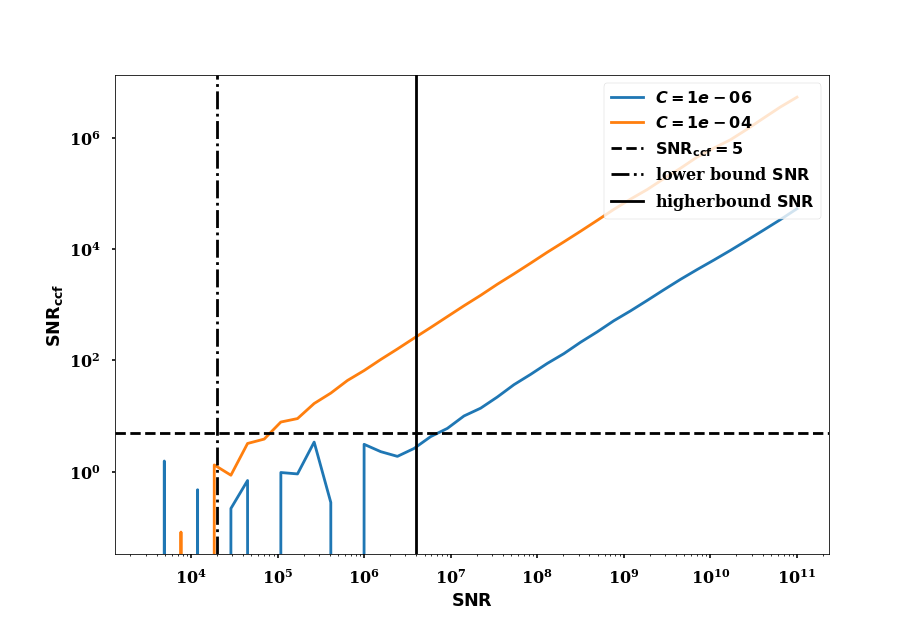
\includegraphics[scale={0.5}]{images/Chapter3/parspace_new.png}}
    \caption{A depiction of the parameter space chosen to test the cross correlation based detection algorithm where the x-axis shows the $\rm{SNR}$ and the y-axis shows the $\rm{SNR_{\rm{ccf}}}$. The different colored lines depict different contrasts and relationship between the $\rm{SNR}$ and $\rm{SNR_{\rm{ccf}}}$.
    The vertical lines indicate the lower bound (dash and dot) and the upper bound (solid) of the $\rm{SNR}$ whereeas the horizontal dashed line indicates the $\rm{SNR_{ccf}}\ge6$.}
    \label{fig:parspace-1}
\end{figure}
On the x-axis is $\rm{SNR}$ and on the y-axis is the $\rm{SNR_{ccf}}$. 
The horizontal dashed line represents the cut off of $\rm{SNR_{ccf}}>6$ which is our cut off.
The orange and blue lines represent those spectra with exoplanets at a contrasts of $10^{-4}$ and $10^{-6}$.
The two vertical lines consist of the upper and lower bound of the $\rm{SNR}$. 
The window between the two vertical lines consists now of spectra where very few exoplanets with a contrast of $10^{-6}$.
An interesting observation is that beyond an $\rm{SNR}>5$ the relationship between $\rm{SNR_{ccf}}$ and $\rm{SNR}$ becomes linear and thus it validates our cut off criterion.

\paragraph{Parameter space selection of $R$:\\}
The parameter space of $R$ is limited by the resolution of the \textsc{BT-SETTL} library itself and hence we limit ourselves to a $R<300,000$. 
We choose a sampling rate of $50$ between $10^{2}$ and $10^{5}$ so that we have a total of $20$ different resolutions for each spectrum.

\subsection{The detection matrix }
The goal of defining the parameter space and designing the algorithm was to produce the detection and characterization matrices.
Given the context here, the detection matrix itself is not very difficult to explain and is indeed somewhat self explanatory. 
However, it is important to still define what each row and column means in the detection matrix for warm Jupiters in Fig~\ref{fig:detmat}
\begin{figure}[!ht]
    \centering
    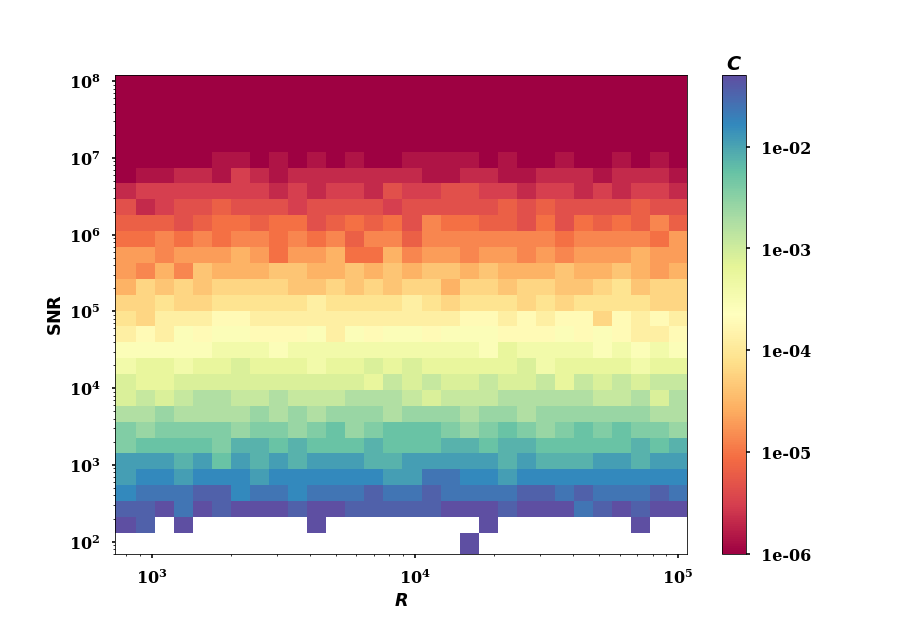
\includegraphics[scale=0.5]{images/Chapter3/detmat.png}
    \caption{The detection matrix presents the detectability of warm Jupiters using their spectra with the cross correlation algorithm. 
    The x-axis is changing $R$ and y-axis is the changing $\rm{SNR}$ and each cell is filled with the contrast at which the warm Jupiter is detectable for a fixed $R$, $\rm{SNR}$.
    This detection matrix is produced for a warm Jupiter with $T_{\rm{eff}}= 1500$~K and $\log(g)=4.5$, but cross correlate the spectra with a template that is $2$ grid points away so as to neither be optimistic or pessimistic with this matrix.
    While this detection matrix is for one kind of exoplanet, this can be repeated for several types of exoplanets and also constructed for specific molecules (i.e narrower wavelength ranges).
    }
    \label{fig:detmat}
\end{figure}
Each cell in the matrix represents a contrast between $10^{-1}$ and $10^{-6}$.
From the bottom to the top the rows represent $\rm{SNR}$ values from the lowest to the highest.
The bottom two rows i.e $\rm{SNR}<300$ contain a lot of white cells, these are cells where even for the unphysically low contrasts of $0.1$ the exoplanets were not detected. 
These $\rm{SNR}$ represent cases where no matter what the $R$ and $C$ are the exoplanet is completely undetectable.
There are many interesting points to note from this detection matrix.
As with Fig~\ref{fig:parspace-1} we saw that a linear relationship exists between the $\rm{SNR_{ccf}}$ and $\rm{SNR}$ which implied that the $\rm{SNR}$ seems to directly influence the cross correlation strength.
The detection matrix seems to reinforce this idea when detecting faint exoplanets.
As the $\rm{SNR}$ increases the matrix gets redder indicating the detectability of fainter companions. 
The top $3$ rows are at a detection limit of $10^{-6}$, this means that the faintest companion is completely detectable for the highest signal to noise of the spectrum.
%For higher values of $R$ and a fixed SNR, there is no significant improvement in the sensitivity of detecting faint exoplanets. Although there are slight improvements at higher SNR, they are washed out when increasing the SNR further. 
%This is because as $R$ increases, $\rm{SNR_{\lambda}}$ decreases, outweighing the advantage of having more wavelength bands. Therefore, for warm Jupiters, increasing $R$ does not provide any noticeable advantage in detection.
\subsection{Characterization error bars }
\label{sec:char error bars}
The characterization of an exoplanet is carried out in two subsequent steps,
\begin{enumerate}
    \item produce the characterization matrix with $\rm{SNR_{ccf}}$ or $LL$ where both the matrices have to be mirror images of each other and
    \item fit the inverse Gaussian to $LL$ characterization matrix.
\end{enumerate}
For the first part, it is important to first look at a sample plots of the characterization matrices at specific values from the parameter space.
We choose a spectrum with a $T_{\rm{eff}}= 1500$ and a $\rm{\log(g)} = 4.5$.
We start with a lower $\rm{SNR}$ where the exoplanet is not detectable in Fig~\ref{fig:nondet_char}.
\begin{figure}[!h]
    \centering
    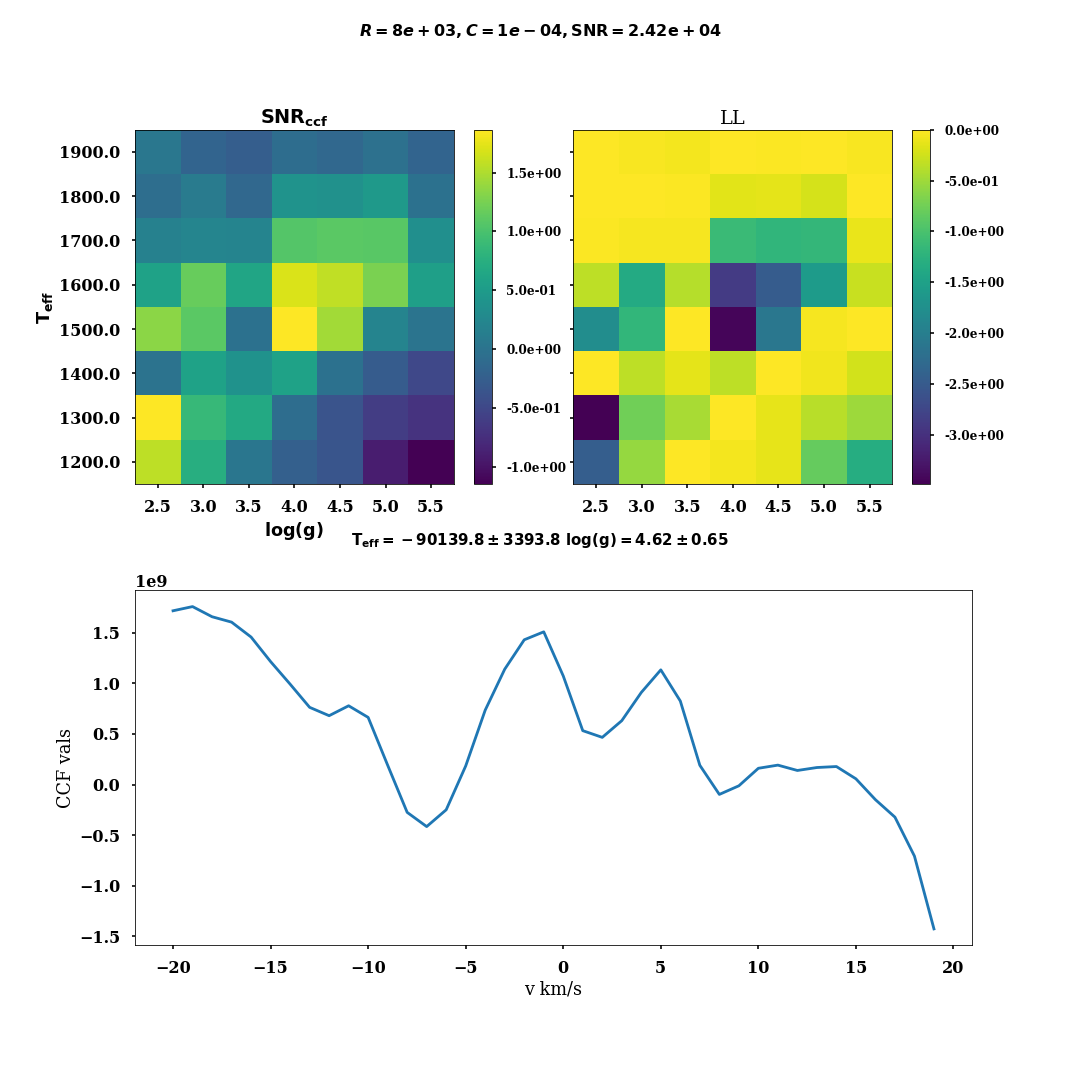
\includegraphics[scale=0.4]{images/Chapter3/char_plots_8e+03_1e-04_2.42e+04.png}
    \caption{We produce a characterization matrix based on the template in Table~\ref{tab:charmat_rep}, the characterization parameter can be either $\rm{SNR_{ccf}}$ (left) or $LL$ (right) and the cross correlation function at $\rm{max~(SNR_{ccf})}$ or $\textrm{min~}(LL)$ is depicted at the bottom.
    This plot shows that we can find the approximate $\log(g)$ but have large error bars in $T_{\rm{eff}}$ when the warm Jupiter cannot be detected (i.e $\rm{SNR_{ccf}}<6$).
    }
    \label{fig:nondet_char}
\end{figure}
The top left is the characterization matrix with $\rm{SNR_{ccf}}$ as the parameter within the matrix and $LL$ as the parameter on the top right.
The bottom of the plot is the shape of the cross correlation function with respect to the velocity.
Note that for the contrast involved this exoplanet is not detectable and appropriately it is not possible to quantify the error bar in the effective temperature.
This also reinforces the idea of having a characterization hypothesis where the exoplanet is characterizable only if an exoplanet is definitely detectable.
Based on Fig~\ref{fig:detmat} as we increase the $\rm{SNR}$ we will be able to detect the exoplanet. 
At $\rm{SNR_{ccf}}<5$ the relationship is still not linear and therefore, it is possible that we don't have enough photons in enough wavelength bins to have a detection and characterization. 
Therefore, we depict a case where $\rm{SNR_{ccf}}>5$ in Fig~\ref{fig:charmap-det}.
\begin{figure}[!h]
    \centering
    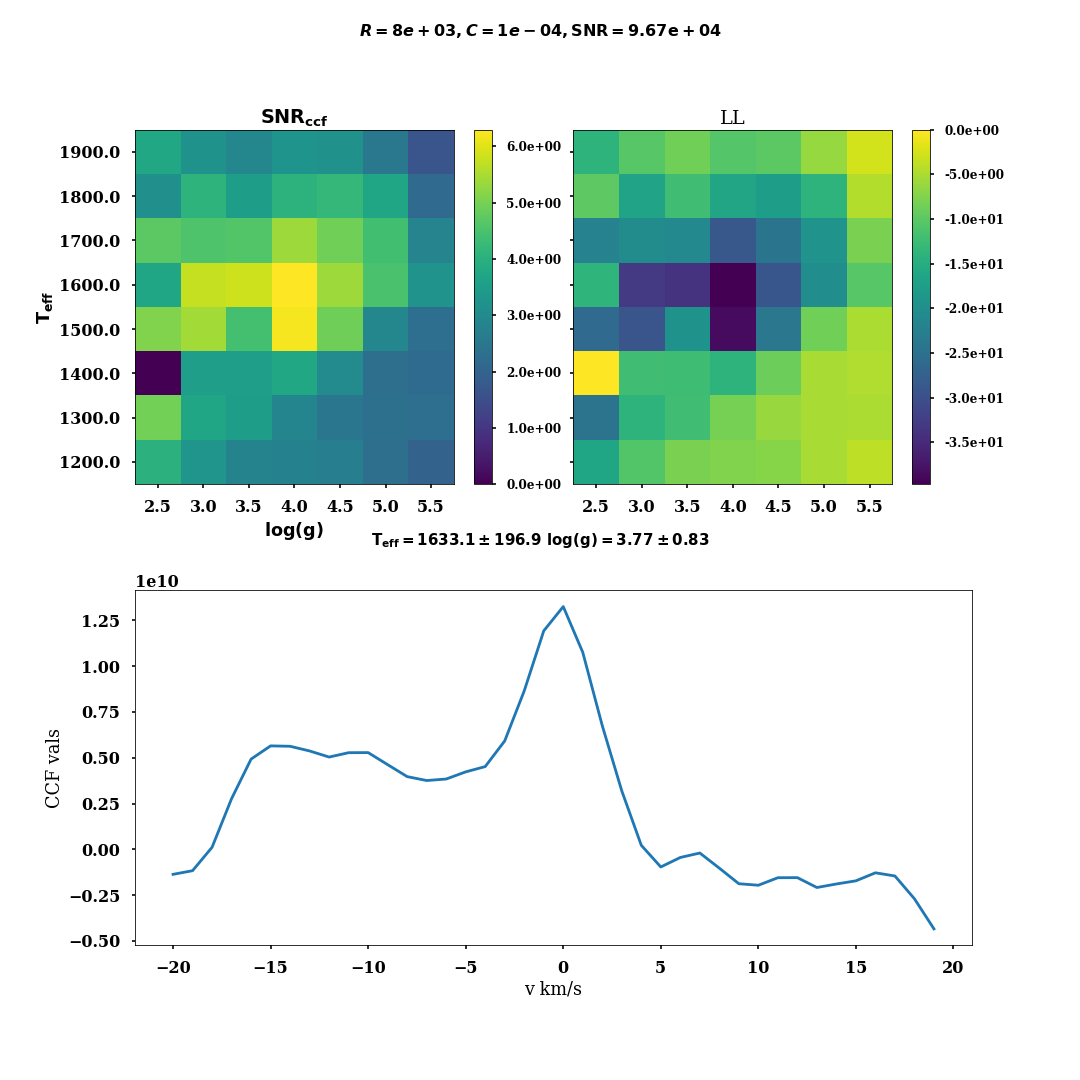
\includegraphics[scale=0.4]{images/Chapter3/char_plots_8e+03_1e-04_9.67e+04.png}
    \caption{In this instance of a characterization matrix, we use a spectrum with a higher SNR where we detect the exoplanet. 
    The error bar is $\approx~200$K and $<0.83$ in $\rm{T_{eff}}$ and $\log(g)$ respectively.
    The cross correlation also peaks clearly at $v=0$ km/s, which are all signs of a well detected exoplanet and thus our characterization is also accurate.}
    \label{fig:charmap-det}
\end{figure}
A couple of interesting points of comparison between these two last figures,
\begin{enumerate}
    \item firstly, when the $\rm{SNR_{ccf}}<6$, it's clear that $T_{\rm{eff}}$ is misestimated and the depth of the $LL$ is shallow. The mean $\log(g)$ is wrong as well. 
    \item Secondly, when $\rm{SNR_{ccf}}\ge ~6$ the $LL$ trough is deeper and thus the characterization is more accurate.
\end{enumerate}
The first question which arises is whether further increase in the $\rm{SNR}$, that showed improved detection sensitivity in Fig \ref{fig:detmat}, will also show increased characterization accuracy.
We answer this question by characterizing two spectra with progressively higher $\rm{SNR}$ in 
Fig~\ref{fig:charmap-deeptrough} and Fig~\ref{fig:highres-charmat}. 
In both these cases the $\rm{SNR_{ccf}}\gg 6$, but notice that there is no improvement to the error bars of both $T_{\rm{eff}}$ and $\log(g)$. 
%This also leads a 'deeper' trough in the $LL$.
\begin{figure}[!ht]
    \centering
    \includegraphics[scale=0.3]{{images/Chapter3/char_plots_1e+05_1e-06_1.85e+07.png}}
    \caption{This is a characterization matrix with the same spectral features but at a higher $\rm{SNR}$ than in Fig~\ref{fig:charmap-det}. 
    The error bars are lower and the mean characterization values are quite close to what is expected. 
    But it is possible that even thought the $\rm{SNR}$ is high the $R$ is still too low to have enough spectral features to reduce the error bar.}
    \label{fig:charmap-deeptrough}
\end{figure}
The spectrum in Fig~\ref{fig:charmap-deeptrough} though has a high $\rm{SNR}$, still is a moderate resolution spectrum, therefore to rule out the possibility that it is the spectral resolution we also test the characterization accuracy with a higher resolution version in Fig~\ref{fig:highres-charmat}.
%However, this does not produce a narrower trough because of the velocity resolution. 
%Consequently, the characterization accuracy does not improve. 
While the $\log(\rm{g})$ is slight above one template resolution unit ($0.5$ dex) the $\rm{T_{eff}}$ has an error bar $\approx~200$K which is twice the resolution unit of $100$K. 
This error bar also is quite close to the error bar at $\rm{SNR}$ where the exoplanet is just detected.
This shows that increasing neither increasing $R$ nor $\rm{SNR}$ produces a more accurate characterization, whereas for detection a higher $\rm{SNR}$ does produce fainter detections.
\begin{figure}[!ht]
    \centering
    \includegraphics[scale=0.3]{images/Chapter3/char_plots_1e+05_1e-06_1.85e+07.png}
    \caption{The same spectrum as from Fig\ref{fig:charmap-deeptrough} but at higher resolution and slightly higher $\rm{SNR}$ because of the increased number $\lambda_N$.}
    \label{fig:highres-charmat}
\end{figure}

It is, thus, clear that there is a theoretical limit to how accurate a characterization can be.
This is not influenced by any parameters beyond the fact that the exoplanet is detectable in the spectrum.
It is also interesting, that the width of the Gaussian of the cross correlation does not get narrower and consequently it appears that the width of the $LL$ is also equally wide.
This width as we have seen defines the $\sigma_x$ which is our error bar.
In the discussion section of this chapter we will define the benchmark that the cross correlation algorithm sets for the ML algorithms and what steps the ML algorithms need to pass to be considered usable for scientific analysis.
\section{Discussion and conclusion}
We end this part with a small discussion which will motivate the use of the imaging dimension along with the spectral dimension to improve detection sensitivity. 